\documentclass[aspectratio=169,11pt]{beamer}
\usepackage[T1]{fontenc}
\usepackage[utf8]{inputenc}
\usepackage[provide=*,french]{babel}
\usepackage{lmodern}
\usepackage{tikz}
\usetikzlibrary{arrows.meta,positioning,calc,shapes.geometric}
\usepackage{listings}
\usepackage{hyperref}
\definecolor{vert}{HTML}{1C322D}
\definecolor{creme}{HTML}{F8F3EE}
\definecolor{or}{HTML}{EBB552}
\definecolor{rose}{HTML}{F1CDBE}
\definecolor{encre}{HTML}{203A34}
\definecolor{bleu}{HTML}{2563A6}
\setbeamercolor{normal text}{fg=creme,bg=vert}
\setbeamercolor{frametitle}{fg=creme,bg=vert}
\setbeamercolor{title}{fg=creme}
\setbeamercolor{structure}{fg=or}
\setbeamercolor{block title}{fg=vert,bg=or}
\setbeamercolor{block body}{fg=vert,bg=creme}
\setbeamercolor{alerted text}{fg=or}
\setbeamertemplate{navigation symbols}{}
\setbeamertemplate{footline}{\hfill\color{creme!60}\scriptsize SNT · Le Web · Séance 3\quad\insertframenumber\,/\,\inserttotalframenumber\hspace{5mm}\vspace{3mm}}
\setbeamertemplate{frametitle}{\vspace{3mm}\insertframetitle\par\vspace{2mm}\color{or}\rule{\linewidth}{.6pt}}
\setbeamersize{text margin left=9mm,text margin right=9mm}
\newcommand{\question}[1]{{\Large\color{or}\bfseries #1}}
\newcommand{\indice}[1]{\vspace{3mm}{\color{rose}\small #1}}
\newcommand{\parole}[1]{\vfill{\color{or}\footnotesize À faire formuler par les élèves : }{\color{creme}\footnotesize #1}}
\newcommand{\noteprof}[1]{\note{#1}}
\tikzset{machine/.style={draw=or,thick,rounded corners=2mm,fill=creme,text=vert,align=center,minimum width=3.2cm,minimum height=1.6cm}, fleche/.style={-{Latex[length=3mm]},thick,draw=or}}
\lstset{basicstyle=\ttfamily\small,breaklines=true,showstringspaces=false,columns=fullflexible,backgroundcolor=\color{creme},frame=single,rulecolor=\color{or},keywordstyle=\color{bleu},commentstyle=\color{encre}}
\title{Qui fait quoi quand on visite une page Web ?}
\subtitle{Client, serveur, HTTP et code exécuté}
\author{SNT · Classe de seconde}
\date{Séance 3 · Support d'explication}
\begin{document}

\begin{frame}[plain]
\vspace{1.1cm}
{\color{or}\large SNT · LE WEB · SÉANCE 3}\par\vspace{6mm}
{\Huge\bfseries Qui fait quoi quand on visite une page Web ?}\par\vspace{7mm}
{\color{rose}\Large Une enquête à partir d'un simple F5}\par
\vfill {\small Client · serveur · HTTP · JavaScript · PHP · DOM}\vspace{7mm}
\end{frame}

\begin{frame}{Le mystère du titre qui disparaît}
\question{Pourquoi ma modification ne reste-t-elle pas ?}
\vspace{5mm}
\begin{center}
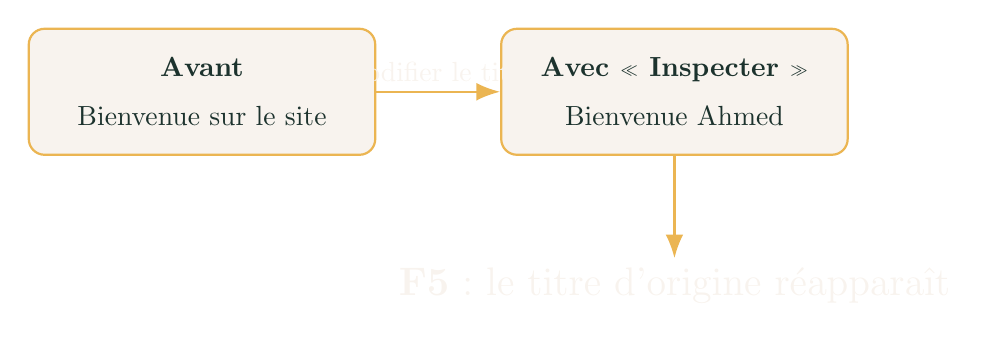
\begin{tikzpicture}
\node[machine,minimum width=4.4cm] (a) at (0,0) {\textbf{Avant}\\[2mm] Bienvenue sur le site};
\node[machine,minimum width=4.4cm] (b) at (6,0) {\textbf{Avec « Inspecter »}\\[2mm] Bienvenue Ahmed};
\draw[fleche] (a)--node[above,text=creme]{modifier le titre}(b);
\node[below=1.3cm of b, text=creme,align=center] (c) {\Large \textbf{F5} : le titre d'origine réapparaît};
\draw[fleche] (b.south)--(c.north);
\end{tikzpicture}
\end{center}
\parole{Où se trouve la version d'origine ? Qui la fournit ?}
\noteprof{Faire rappeler l'activité 2.1. Laisser formuler deux ou trois hypothèses avant de poursuivre. Ne pas affirmer que F5 retélécharge toujours tout : le cache existe.}
\end{frame}

\begin{frame}{Une page pour plusieurs visiteurs}
\question{Si toute la page était seulement chez moi...}
\vspace{6mm}
\begin{itemize}\setlength{\itemsep}{6mm}
\item Comment mon voisin pourrait-il consulter la même page ?
\item Comment le site pourrait-il être disponible demain ?
\item Qui conserverait la version de référence ?
\end{itemize}
\pause
\vspace{4mm}
\begin{block}{Idée construite ensemble}
Une machine accessible par le réseau fournit la ressource demandée : c'est le \textbf{serveur}. Mon navigateur joue le rôle de \textbf{client}.
\end{block}
\noteprof{Faire émerger le besoin d'une ressource accessible. Un serveur désigne un rôle/service, pas nécessairement une machine unique toujours allumée. Trace écrite : section 9.}
\end{frame}

\begin{frame}{Le dialogue client–serveur}
\question{Comment demander la page ?}
\vspace{6mm}
\begin{center}
\begin{tikzpicture}
\node[machine] (c) at (0,0) {\textbf{CLIENT}\\ Navigateur};
\node[machine] (s) at (8,0) {\textbf{SERVEUR}\\ Site Web};
\only<2->{\draw[fleche] ([yshift=5mm]c.east)--node[above,text=creme,align=center]{\textbf{REQUÊTE}\\ « Je veux /index.html »}([yshift=5mm]s.west);}
\only<3->{\draw[fleche] ([yshift=-5mm]s.west)--node[below,text=creme,align=center]{\textbf{RÉPONSE}\\ « 200 OK » + HTML}([yshift=-5mm]c.east);}
\end{tikzpicture}
\end{center}
\vspace{8mm}
\only<1>{\centering Émettre une hypothèse : qui parle en premier ?}
\only<2>{\centering Le client prend l'initiative de demander.}
\only<3->{\centering Le serveur répond à la demande.}
\noteprof{Afficher les flèches séparément. Faire verbaliser les deux sens. Un site peut charger plusieurs fichiers et contacter plusieurs serveurs.}
\end{frame}

\begin{frame}{Pourquoi faut-il des règles communes ?}
\question{Comment le serveur comprend-il la demande ?}
\vspace{4mm}
\begin{columns}[T]
\column{.47\linewidth}
\begin{block}{Demande floue}
« Bonjour, je voudrais la page, s'il vous plaît... »
\end{block}
\column{.47\linewidth}
\pause
\begin{block}{Demande structurée}
\texttt{GET /index.html HTTP/1.1}
\end{block}
\end{columns}
\pause
\vspace{8mm}
\begin{center}
{\Large \textbf{HTTP} = un protocole}\par\smallskip
Un ensemble de règles pour formuler les \textbf{requêtes} et les \textbf{réponses}.
\end{center}
\parole{À quoi sert le mot GET ? Et /index.html ?}
\end{frame}

\begin{frame}{La requête HTTP, pièce par pièce}
\question{Que signifie chaque morceau ?}
\vspace{4mm}
\begin{center}
\begin{tikzpicture}[every node/.style={font=\ttfamily\Large}]
\node[fill=or,text=vert,rounded corners,inner sep=5pt] (m) at (0,0) {GET};
\node[fill=creme,text=vert,rounded corners,inner sep=5pt] (p) at (4,0) {/search?q=snt};
\node[fill=rose,text=vert,rounded corners,inner sep=5pt] (v) at (8.3,0) {HTTP/1.1};
\only<2->{\node[below=1.2cm of m,text=creme,font=\normalsize,align=center] {Méthode\\ (action)};}
\only<3->{\node[below=1.2cm of p,text=creme,font=\normalsize,align=center] {Ressource\\ + paramètres};}
\only<4->{\node[below=1.2cm of v,text=creme,font=\normalsize,align=center] {Version du\\ protocole};}
\end{tikzpicture}
\end{center}
\vfill
\only<5->{\begin{block}{Autre exemple} \texttt{POST} sert souvent à envoyer les données d'un formulaire dans le corps de la requête. \textbf{POST ne chiffre pas les données.}\end{block}}
\noteprof{Lire la ligne de gauche à droite. Expliquer que GET peut avoir des paramètres dans l'URL et que POST peut également avoir des paramètres d'URL. HTTPS protège la transmission.}
\end{frame}

\begin{frame}[fragile]{Des renseignements accompagnent la demande}
\question{Que peut apprendre le serveur ?}
\vspace{3mm}
\begin{lstlisting}
GET /search?q=snt+seconde&lang=fr HTTP/1.1
Host: www.moteur.fr
User-Agent: Firefox/128.0
Accept-Language: fr-FR
Cookie: session=a8f3e2
\end{lstlisting}
\pause
\vspace{3mm}
{\color{or}\bfseries En-têtes HTTP}\quad Nom du site, logiciel utilisé, langue préférée, cookie éventuellement présent.
\parole{Quelles informations avons-nous données volontairement ?}
\noteprof{Le bloc est un exemple simplifié, inspiré du document 12. Ne pas déduire l'identité de la personne du seul User-Agent.}
\end{frame}

\begin{frame}{La réponse du serveur}
\question{Comment savoir si la demande a réussi ?}
\vspace{5mm}
\begin{center}
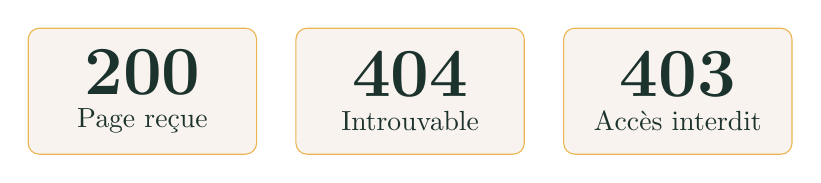
\begin{tikzpicture}
\foreach \x/\n/\lab in {0/200/Page reçue,3.4/404/Introuvable,6.8/403/Accès interdit}{
 \node[draw=or,fill=creme,text=vert,rounded corners,minimum width=2.9cm,minimum height=1.6cm,align=center] at (\x,0) {\Huge\bfseries \n\\\normalsize \lab};
}
\end{tikzpicture}
\end{center}
\pause
\vspace{7mm}
\begin{block}{Une réponse HTTP contient}
Un \textbf{code d'état}, des \textbf{en-têtes} (ex. \texttt{Content-Type: text/html}) et, souvent, un \textbf{corps} contenant la ressource.
\end{block}
\noteprof{Mentionner 301 (redirection) et 500 (erreur du serveur) à l'oral sans surcharger. Trace écrite : section 10.}
\end{frame}

\begin{frame}{Le paradoxe de la connexion}
\question{Comment un site se souvient-il de moi ?}
\vspace{4mm}
\begin{itemize}\setlength{\itemsep}{4mm}
\item Je me connecte au site.
\item Je clique ensuite sur « Mon compte ».
\item Le serveur reçoit une \textbf{nouvelle} requête HTTP.
\end{itemize}
\pause
\vspace{4mm}
\begin{block}{Une solution : le cookie}
Le serveur peut demander au navigateur de conserver une petite \textbf{donnée}. Pour des requêtes ultérieures compatibles avec ses règles, le navigateur la renvoie.
\end{block}
\parole{Pourquoi cela aide-t-il le serveur à reconnaître une session ?}
\noteprof{Expliquer oralement la question 3.1 d. Nuancer : les cookies ne sont pas forcément des fichiers distincts, et leur renvoi dépend du domaine, du chemin et des attributs du cookie.}
\end{frame}

\begin{frame}{Deux requêtes, une session}
\vspace{4mm}
\begin{center}
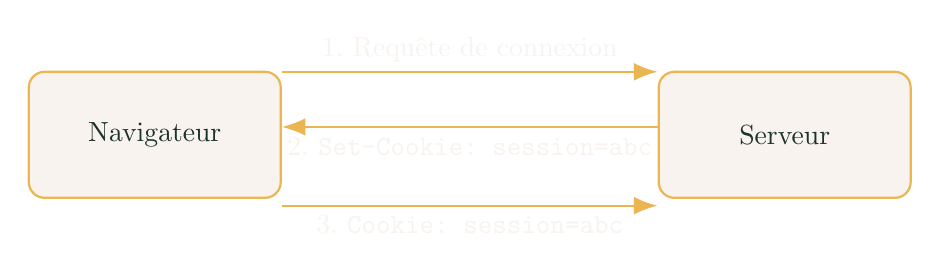
\begin{tikzpicture}
\node[machine] (c) at (0,0) {Navigateur};
\node[machine] (s) at (8,0) {Serveur};
\draw[fleche] ([yshift=8mm]c.east)--node[above,text=creme]{1. Requête de connexion}([yshift=8mm]s.west);
\pause
\draw[fleche] ([yshift=1mm]s.west)--node[below,text=creme,align=center]{2. \texttt{Set-Cookie: session=abc}}([yshift=1mm]c.east);
\pause
\draw[fleche] ([yshift=-9mm]c.east)--node[below,text=creme,align=center]{3. \texttt{Cookie: session=abc}}([yshift=-9mm]s.west);
\end{tikzpicture}
\end{center}
\vspace{10mm}
\only<3->{\centering Le cookie peut servir d'\textbf{identifiant de session}.}
\noteprof{Important : la reconnaissance repose aussi sur une session côté serveur. Les mécanismes de sécurité réels sont plus complexes.}
\end{frame}

\begin{frame}{Passage à l'activité 3.1}
\question{Peux-tu lire une vraie structure HTTP ?}
\vspace{8mm}
\begin{enumerate}\setlength{\itemsep}{5mm}
\item Repère la méthode et le chemin.
\item Décode les paramètres \texttt{q} et \texttt{lang}.
\item Repère trois informations envoyées dans les en-têtes.
\item Pour \texttt{Set-Cookie}, nous construirons la réponse ensemble.
\end{enumerate}
\vfill
\begin{center}{\Large\color{or}\bfseries Livret 3 · Activité 3.1}\end{center}
\end{frame}

\begin{frame}{Une page, combien de requêtes ?}
\question{Une seule page Web = une seule requête ?}
\vspace{6mm}
\begin{center}
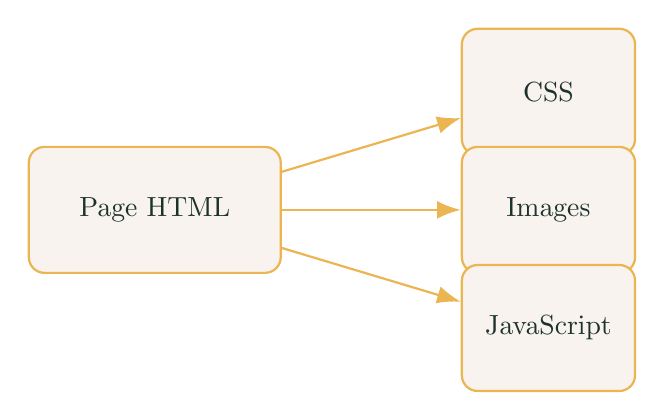
\begin{tikzpicture}
\node[machine] (p) at (0,0) {Page HTML};
\only<2->{\node[machine,minimum width=2.2cm] (css) at (5,1.5) {CSS};\node[machine,minimum width=2.2cm] (img) at (5,0) {Images};\node[machine,minimum width=2.2cm] (js) at (5,-1.5) {JavaScript};
\draw[fleche] (p)--(css); \draw[fleche] (p)--(img); \draw[fleche] (p)--(js);}
\end{tikzpicture}
\end{center}
\vspace{3mm}{\color{or}\small Question aux élèves : }\small Combien de lignes verrons-nous dans Firefox ?
\noteprof{Les ressources peuvent provenir de plusieurs domaines. Certains fichiers peuvent venir du cache, et des ressources peuvent être chargées plus tard.}
\end{frame}

\begin{frame}{Firefox : voir le réseau en action}
\question{Où observer les requêtes ?}
\vspace{7mm}
\begin{enumerate}\setlength{\itemsep}{7mm}
\item Ouvrir le site dans \textbf{Firefox}.
\item Appuyer sur \textbf{F12}, puis choisir \textbf{Réseau}.
\item Recharger avec \textbf{F5}.
\item Lire les colonnes \textbf{État}, \textbf{Méthode}, \textbf{Domaine}, \textbf{Type}.
\end{enumerate}
\vfill
\begin{center}{\Large\color{or}\bfseries Livret 3 · Activité 3.2}\end{center}
\noteprof{Faire une démonstration de 30 secondes. Sélectionner la ligne de type HTML, puis les En-têtes pour lire Content-Type. Les valeurs changent d'un poste à l'autre.}
\end{frame}

\begin{frame}{Une page peut réagir sans recharger}
\question{Qui affiche « champ obligatoire » ?}
\vspace{6mm}
\begin{center}
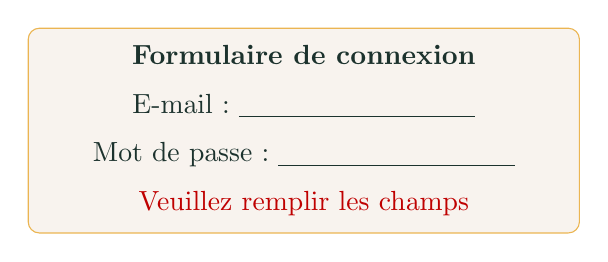
\begin{tikzpicture}
\node[draw=or,fill=creme,text=vert,rounded corners,minimum width=7cm,minimum height=2.6cm,align=center] (f) {
\textbf{Formulaire de connexion}\\[2mm]
E-mail : \underline{\hspace{3cm}}\\[2mm]
Mot de passe : \underline{\hspace{3cm}}\\[2mm]
\textcolor{red!75!black}{Veuillez remplir les champs}
};
\end{tikzpicture}
\end{center}
\pause
\begin{block}{Hypothèse à vérifier}
Un programme exécuté \textbf{dans le navigateur} peut réagir immédiatement à une action. Ici, le \textbf{JavaScript} contrôle le formulaire.
\end{block}
\noteprof{Faire cliquer sur « Se connecter » avec champs vides dans connexion.html. Le code spécifique de la démonstration empêche alors l'envoi. Le simple fait de ne pas recharger n'est pas une preuve universelle d'absence de réseau.}
\end{frame}

\begin{frame}{JavaScript et PHP : deux lieux d'exécution}
\question{Qui exécute le programme ?}
\vspace{7mm}
\begin{center}

\begin{tikzpicture}
\node[machine,minimum width=4cm,minimum height=2.2cm] (c) at (0,0) {\textbf{NAVIGATEUR}\\[2mm] HTML + CSS\\\textbf{JavaScript}};
\node[machine,minimum width=4cm,minimum height=2.2cm] (s) at (7.7,0) {\textbf{SERVEUR}\\[2mm] \textbf{PHP}\\ données};
\draw[fleche] ([yshift=4mm]c.east)--node[above,text=creme]{requête}([yshift=4mm]s.west);
\draw[fleche] ([yshift=-4mm]s.west)--node[below,text=creme]{résultat, ex. HTML}([yshift=-4mm]c.east);
\end{tikzpicture}
\end{center}
\pause
\vspace{5mm}
\begin{block}{Point essentiel}
\textbf{Ctrl+U} peut montrer le JavaScript fourni au navigateur. Sur un serveur PHP normalement configuré, le visiteur reçoit le \textbf{résultat}, pas le source PHP.
\end{block}
\end{frame}

\begin{frame}{Pourquoi vérifier côté serveur ?}
\question{Et si le navigateur mentait ?}
\vspace{5mm}
\begin{itemize}\setlength{\itemsep}{5mm}
\item Le JavaScript peut avertir : « mot de passe manquant ».
\pause
\item Mais l'utilisateur contrôle son navigateur et peut modifier son comportement.
\pause
\item Le serveur doit donc \textbf{vérifier lui-même} les données sensibles.
\end{itemize}
\vspace{5mm}
\begin{block}{Exemple}
Le navigateur améliore l'expérience de saisie. Le serveur décide si l'authentification est autorisée.
\end{block}
\noteprof{Faire imaginer un contrôle uniquement dans le navigateur. Éviter de prétendre que tout traitement de données personnelles est toujours côté serveur.}
\end{frame}

\begin{frame}{Le DOM : la page représentée en mémoire}
\question{Qu'a modifié l'outil « Inspecter » ?}
\vspace{3mm}
\begin{center}
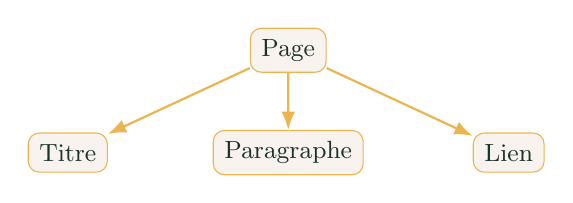
\begin{tikzpicture}[level distance=13mm,sibling distance=28mm,
 every node/.style={draw=or,rounded corners,fill=creme,text=vert,font=\small,inner sep=4pt},
 edge from parent/.style={draw=or,thick,-{Latex}}]
\node {Page}
 child {node {Titre}}
 child {node {Paragraphe}}
 child {node {Lien}};
\end{tikzpicture}
\end{center}
\pause
\vspace{4mm}
\begin{block}{DOM}
Le navigateur construit une représentation des éléments de la page. « Inspecter » peut modifier cette représentation \textbf{locale}, sans changer le fichier d'origine sur le serveur.
\end{block}
\parole{Pourquoi mon voisin ne voit-il pas le nouveau titre ?}
\end{frame}

\begin{frame}{Passage aux activités 3.3 et 3.4}
\question{Peux-tu retrouver les deux côtés ?}
\vspace{6mm}
\begin{enumerate}\setlength{\itemsep}{5mm}
\item \textbf{3.3} : tester \texttt{connexion.html} et lire \texttt{<script>}.
\item Repérer \texttt{<form>}, \texttt{action} et \texttt{method}.
\item Ouvrir la \textbf{copie locale} de \texttt{connexion.php}.
\item \textbf{3.4} : classer chaque opération côté client ou serveur, avec une justification.
\end{enumerate}
\noteprof{Le fichier PHP local est lisible car l'élève en possède une copie. Sans serveur PHP, il ne s'exécute pas simplement en ouvrant le fichier depuis le disque.}
\end{frame}

\begin{frame}{Vérification rapide}
\question{Quelle affirmation est correcte ?}
\vspace{5mm}
\begin{enumerate}[A.]\setlength{\itemsep}{5mm}
\item POST chiffre automatiquement les mots de passe.
\item Modifier le DOM change le site pour tous les visiteurs.
\item Le navigateur peut envoyer une requête GET à un serveur.
\end{enumerate}
\pause
\vspace{6mm}
\begin{block}{Réponse : C}
POST ne chiffre pas. Une modification locale du DOM ne modifie pas la page des autres utilisateurs. Le navigateur peut envoyer une requête \texttt{GET}.
\end{block}
\noteprof{Faire voter A/B/C avant l'apparition de la réponse.}
\end{frame}

\begin{frame}{Le modèle à retenir}
\begin{center}
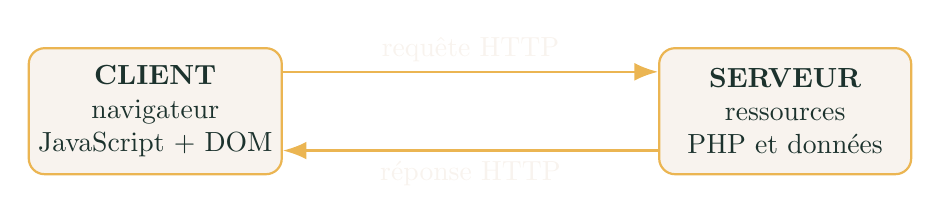
\begin{tikzpicture}
\node[machine] (c) at (0,0) {\textbf{CLIENT}\\ navigateur\\ JavaScript + DOM};
\node[machine] (s) at (8,0) {\textbf{SERVEUR}\\ ressources\\ PHP et données};
\draw[fleche] ([yshift=5mm]c.east)--node[above,text=creme]{requête HTTP}([yshift=5mm]s.west);
\draw[fleche] ([yshift=-5mm]s.west)--node[below,text=creme]{réponse HTTP}([yshift=-5mm]c.east);
\end{tikzpicture}
\end{center}
\vspace{8mm}
\begin{center}
{\Large\color{or}Le navigateur demande. Le serveur répond.}\par\vspace{3mm}
Le code peut s'exécuter \textbf{de part et d'autre}.
\end{center}
\noteprof{Retour à l'énigme de départ : F5 restaure une représentation issue de la ressource et/ou du cache, pas de l'édition locale faite avec Inspecter.}
\end{frame}
\end{document}
